\documentclass{article}
\usepackage[utf8]{inputenc}
\usepackage[brazilian]{babel}
\usepackage{geometry}
\geometry{a4paper, total={150mm,240mm}, top=25mm}
\usepackage{graphicx}
\usepackage{titling}
\usepackage{algorithm}
\usepackage{algpseudocode}
\usepackage{float}
\usepackage{tabularx}
\usepackage{geometry}
\usepackage{rotating}

\title{Exercício Prático 3 - Representação de malhas de triângulos}
\author{Kleyton da Costa (2312730)}
\date{\today}
 
\usepackage{fancyhdr}
\fancypagestyle{plain}{%  the preset of fancyhdr 
    \fancyhf{} % clear all header and footer fields
    \fancyfoot[R]{
\includegraphics[width=3cm]{di.png}}
    \fancyfoot[L]{\today}
    \fancyhead[L]{Geometria Computacional}
    \fancyhead[R]{\theauthor}
}
\makeatletter
\def\@maketitle{%
  \newpage
  \null
  \vskip 1em%
  \begin{center}%
  \let \footnote \thanks
    {\LARGE \@title \par}%
    \vskip 1em%
    %{\large \@date}%
  \end{center}%
  \par
  \vskip 1em}
\makeatother

\begin{document}

\maketitle

\noindent\begin{tabular}{@{}ll}
    Aluno & \theauthor \\
    Professor &  Waldemar Celes (DI/PUC-Rio)
\end{tabular}

\section{Introdução}

Este relatório tem como finalidade apresentar os resultados de aplicação para a representação de malhas de triângulos através de um grafo dual.

\section{Metodologia}

\begin{algorithm}
  \caption{Transform to Dual}
  \label{alg:transform}
  \begin{algorithmic}[1]
  \Procedure{TransformToDual}{$n, m, v, t$}
  \State $dualGraph \gets list()$
  \For{$i \gets 0$ to $n-1$}
  \State $vertexInfo \gets vertices[i] + (-1)$
  \For{$j \gets 0$ to $m-1$}
  \If{$i$ in $t[j]$}
  \State $adjacentTriangule \gets [t$ for $t$ in $t[j]$ if $t \neq i]$
  \State $vertexInfo \gets vertexInfo + tuple(adjacentTriangule)$
  \EndIf
  \EndFor
  \State $dualGraph.append(vertexInfo)$
  \EndFor
  \State \Return $dualGraph$
  \EndProcedure
  \end{algorithmic}
\end{algorithm}

O Algoritmo \ref{alg:transform} possui quatro elementos de entrada: o número de vértices ($n$); o número de triângulos ($m$); a lista de vértices ($v$); e a lista de triângulos ($t$). O algoritmo inicia com uma lista vazia \textit{dualGraph} para realizar o armazenamento da representação do grafo dual. Depois os seguintes passos são executados:

\begin{itemize}
  \item iteração sobre cada vértice de 0 até $n-1$. Para cada vértice, inicializa-se \textit{vertexInfo} através da concatenação das coordenadas do vértice presente na lista $v$ com $-1$, indicando que de início o vértice não possui um triângulo adjacente;
  \item o segundo loop itera de 0 até \textit{m-1}. Para cada triângulo, checa-se se o vértice atual é parte do triângulo utilizando o operador \textit{in}. Se o vértice for encontrado no triângulo, uma lista chamada \textit{adjacentTriangule} é criada iterando sobre os vértices do triângulo e excluindo o vértice atual. Essa lista possui o triângulo adjacente do vértice atual;
  \item Após o loop, o \textit{vertexInfo} é atualizado por uma concatenação com a lista de \textit{adjacentTriangule}. Por fim, o \textit{vertexInfo} é anexado a lista \textit{dualGraph};
  \item Uma vez que todos os vértices forem processados, o algoritmo retorna a lista \textit{dualGraph} - sendo esta a representação do grafo dual.
\end{itemize}

A complexidade do pseudocóidigo é de ordem $O(nm)$, em que $n$ é o número de vértices e $m$ é o número de triângulos. A justificativa é de que o primeiro loop itera $n$ vezes e o segundo loop itera $m$ vezes. Dentro dos loops as operações (concatenação de listas e tuplas, a utilização do operador \textit{in} e iterar sobre os vértices do triângulo) são constantes.  

\section{Experimentos}

Através da malha de triângulos disponibilizada, chegamos no seguinte grafo dual (Figura \ref{fig:grafo_dual}).

\begin{figure}[H]
  \label{fig:grafo_dual}
  \centering
  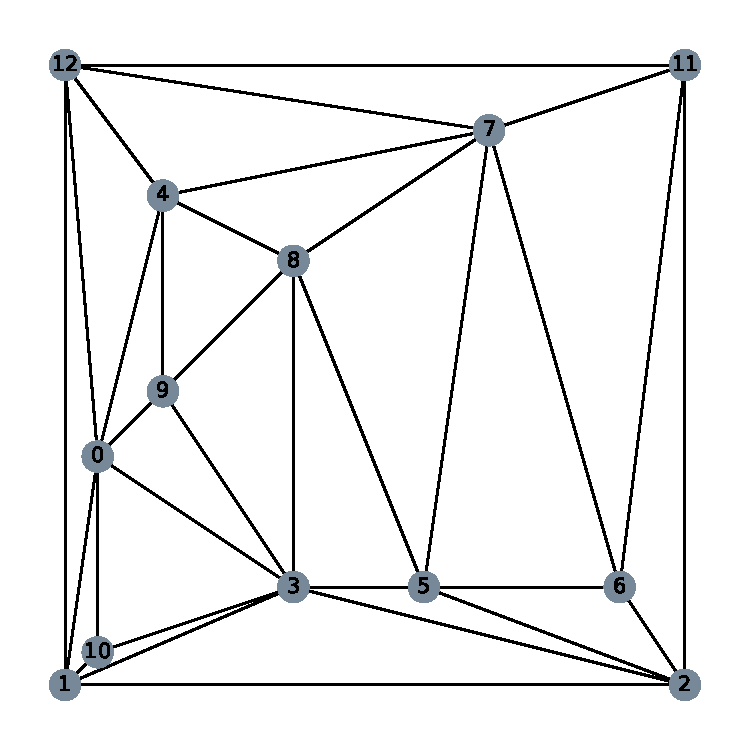
\includegraphics[scale=0.7]{grafo_dual.pdf}
\end{figure}

Cada linha na Tabela \ref{tab:malha} é uma lista contendo informações sobre um vértice e seus triângulos adjacentes.

\begin{sidewaystable}
  \centering
  \label{tab:malha}
  \caption{Informações da malha}
  \begin{tabular}{cccccccccccccccccccccccccccccccc}
  \hline
  \textbf{n} & \textbf{m} & \textbf{t's} &  &  &  &  &  &  &  &  &  &  &  & \\
  \hline
  100.0 & 400.0 & -1 & 1 & 10 & 1 & 12 & 3 & 9 & 4 & 12 & 4 & 9 & 3 & 10 \\
  \hline
  50.0 & 50.0 & -1 & 0 & 10 & 0 & 12 & 2 & 3 & 3 & 10 & -1 & 0 & 10 & 0 & 12 & 2 & 3 & 3 & 10 \\
  \hline
  1000.0 & 50.0 & -1 & 1 & 3 & 3 & 5 & 5 & 6 & 6 & 11 & -1 & 1 & 3 & 3 & 5 & 5 & 6 & 6 & 11 \\
  \hline
  400.0 & 200.0 & -1 & 0 & 9 & 1 & 2 & 2 & 5 & 8 & 9 & 5 & 8 & 1 & 10 & 0 & 10 & -1 & 0 & 9 & 1 & 2 & 2 & 5 & 8 & 9 & 5 & 8 & 1 & 10 & 0 & 10 \\
  \hline
  200.0 & 800.0 & -1 & 0 & 12 & 7 & 12 & 7 & 8 & 0 & 9 & 8 & 9 & -1 & 0 & 12 & 7 & 12 & 7 & 8 & 0 & 9 & 8 & 9 \\
  \hline
  600.0 & 200.0 & -1 & 3 & 2 & 3 & 8 & 2 & 6 & 6 & 7 & 7 & 8 & -1 & 3 & 2 & 3 & 8 & 2 & 6 & 6 & 7 & 7 & 8 \\
  \hline
  900.0 & 200.0 & -1 & 5 & 2 & 5 & 7 & 2 & 11 & 7 & 11 & -1 & 5 & 2 & 5 & 7 & 2 & 11 & 7 & 11 \\
  \hline
  700.0 & 900.0 & -1 & 5 & 6 & 4 & 12 & 5 & 8 & 4 & 8 & 6 & 11 & 11 & 12 & -1 & 5 & 6 & 4 & 12 & 5 & 8 & 4 & 8 & 6 & 11 & 11 & 12 \\
  \hline
  400.0 & 700.0 & -1 & 3 & 9 & 3 & 5 & 5 & 7 & 7 & 4 & 4 & 9 & -1 & 3 & 9 & 3 & 5 & 5 & 7 & 7 & 4 & 4 & 9 \\
  \hline
  200.0 & 500.0 & -1 & 0 & 3 & 3 & 8 & 4 & 0 & 8 & 4 & -1 & 0 & 3 & 3 & 8 & 4 & 0 & 8 & 4 \\
  \hline
  100.0 & 100.0 & -1 & 0 & 1 & 1 & 3 & 3 & 0 & -1 & 0 & 1 & 1 & 3 & 3 & 0 \\
  \hline
  1000.0 & 1000.0 & -1 & 6 & 2 & 7 & 6 & 7 & 12 & -1 & 6 & 2 & 7 & 6 & 7 & 12 \\
  \hline
  50.0 & 1000.0 & -1 & 1 & 0 & 0 & 4 & 4 & 7 & 7 & 11 & -1 & 1 & 0 & 0 & 4 & 4 & 7 & 7 & 11 \\
  \hline
  \end{tabular}
  \end{sidewaystable}
  
O experimento realizado (Figura \ref{fig:experimento}) mostra que, como esperado, o tempo de execução do algoritmo cresce linearmente em função do produto entre o número de vértices e triângulos. Para este experimento foram consideradas 100 amostras com tamanho de entrada $n=100~to~10100$.

\begin{figure}[H]
  \label{fig:experimento}
  \centering
  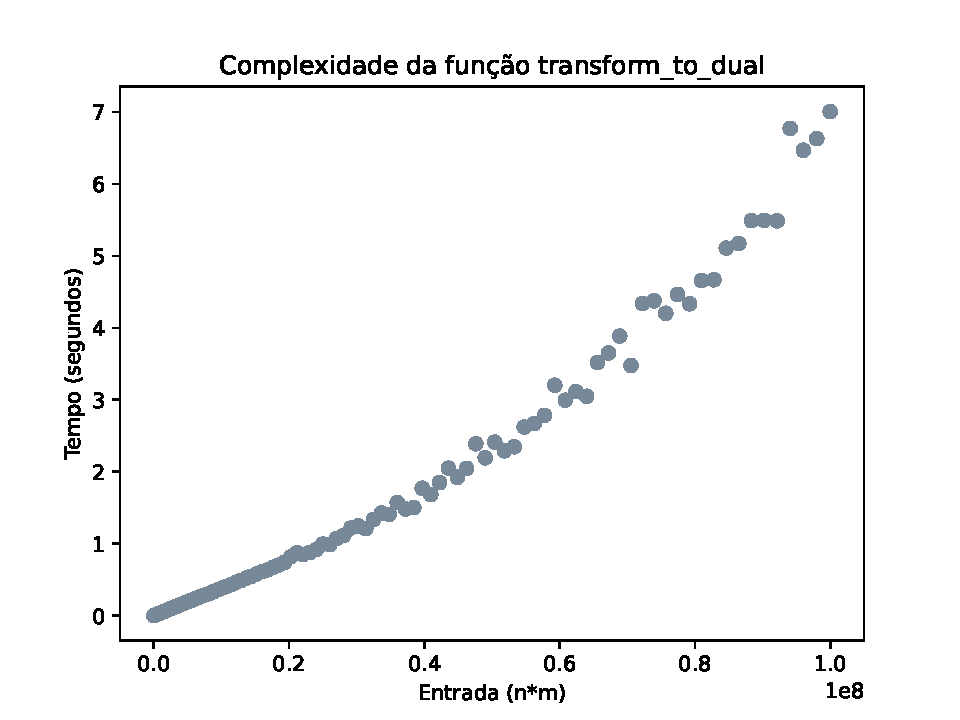
\includegraphics[scale=0.7]{complexidade.pdf}
\end{figure}



\end{document}